\chapter{Конструкция безвинтового подводного робота с внутренними роторами}\label{ch:ch3}

В данной главе описана конструкция безвинтового подводного робота с внутренними роторами. Представлена кинематическая схема, описаны основные элементы конструкции, представлен состав системы управления и описаны ее основные элементы.



\section{Описание конструкции безвинтового подводного робота с внутренними роторами}

Исследования математической модели движения показали, что конструкция безвинтового подводного робота с внутренними роторами должна соответствовать следующим требованиям:

\begin{itemize}
	\item Перпендикулярность роторов.
	\item Для создания максимального эффекта момент инерции роторов должен быть максимальным.
	\item Центр масс всей системы должен быть расположен максимально близко к геометрическому центру эллипсоида.
	\item Форма робота в виде винтового тела --- эллипсоид вращения + винтовые лопасти.
\end{itemize}

Для минимального отклонения центра масс от геометрического центра эллипсоида вместо каждого ротора будем использовать пару роторов. В каждой паре роторы должны быть равноудалены от центра эллипсоида и распологаться на осях эллипсоида.

Безвинтовой подводный робот является мобильным роботом в форме эллипсоида вращения с лопастями и представляет собой сборную конструкцию (рисунок \ref{constr_BPR}). Основой конструкции является оболочка, составленная из двух одинаковых половин 1, присоединенных друг к другу по экваториальной плоскости с помощью дискообразной перегородки – платформы 2. К оболочке крепятся лопасти 3. Размер эллипсоида по большей оси составляет 300 мм, по меньшей – 200 мм. Толщина оболочки (3 мм) и применяемый материал обеспечивают необходимую прочность при погружении и перемещении робота. Соединение полуоболочек и платформы обеспечивает герметичность внутренней полости.

\begin{figure}[h]
	\centering
	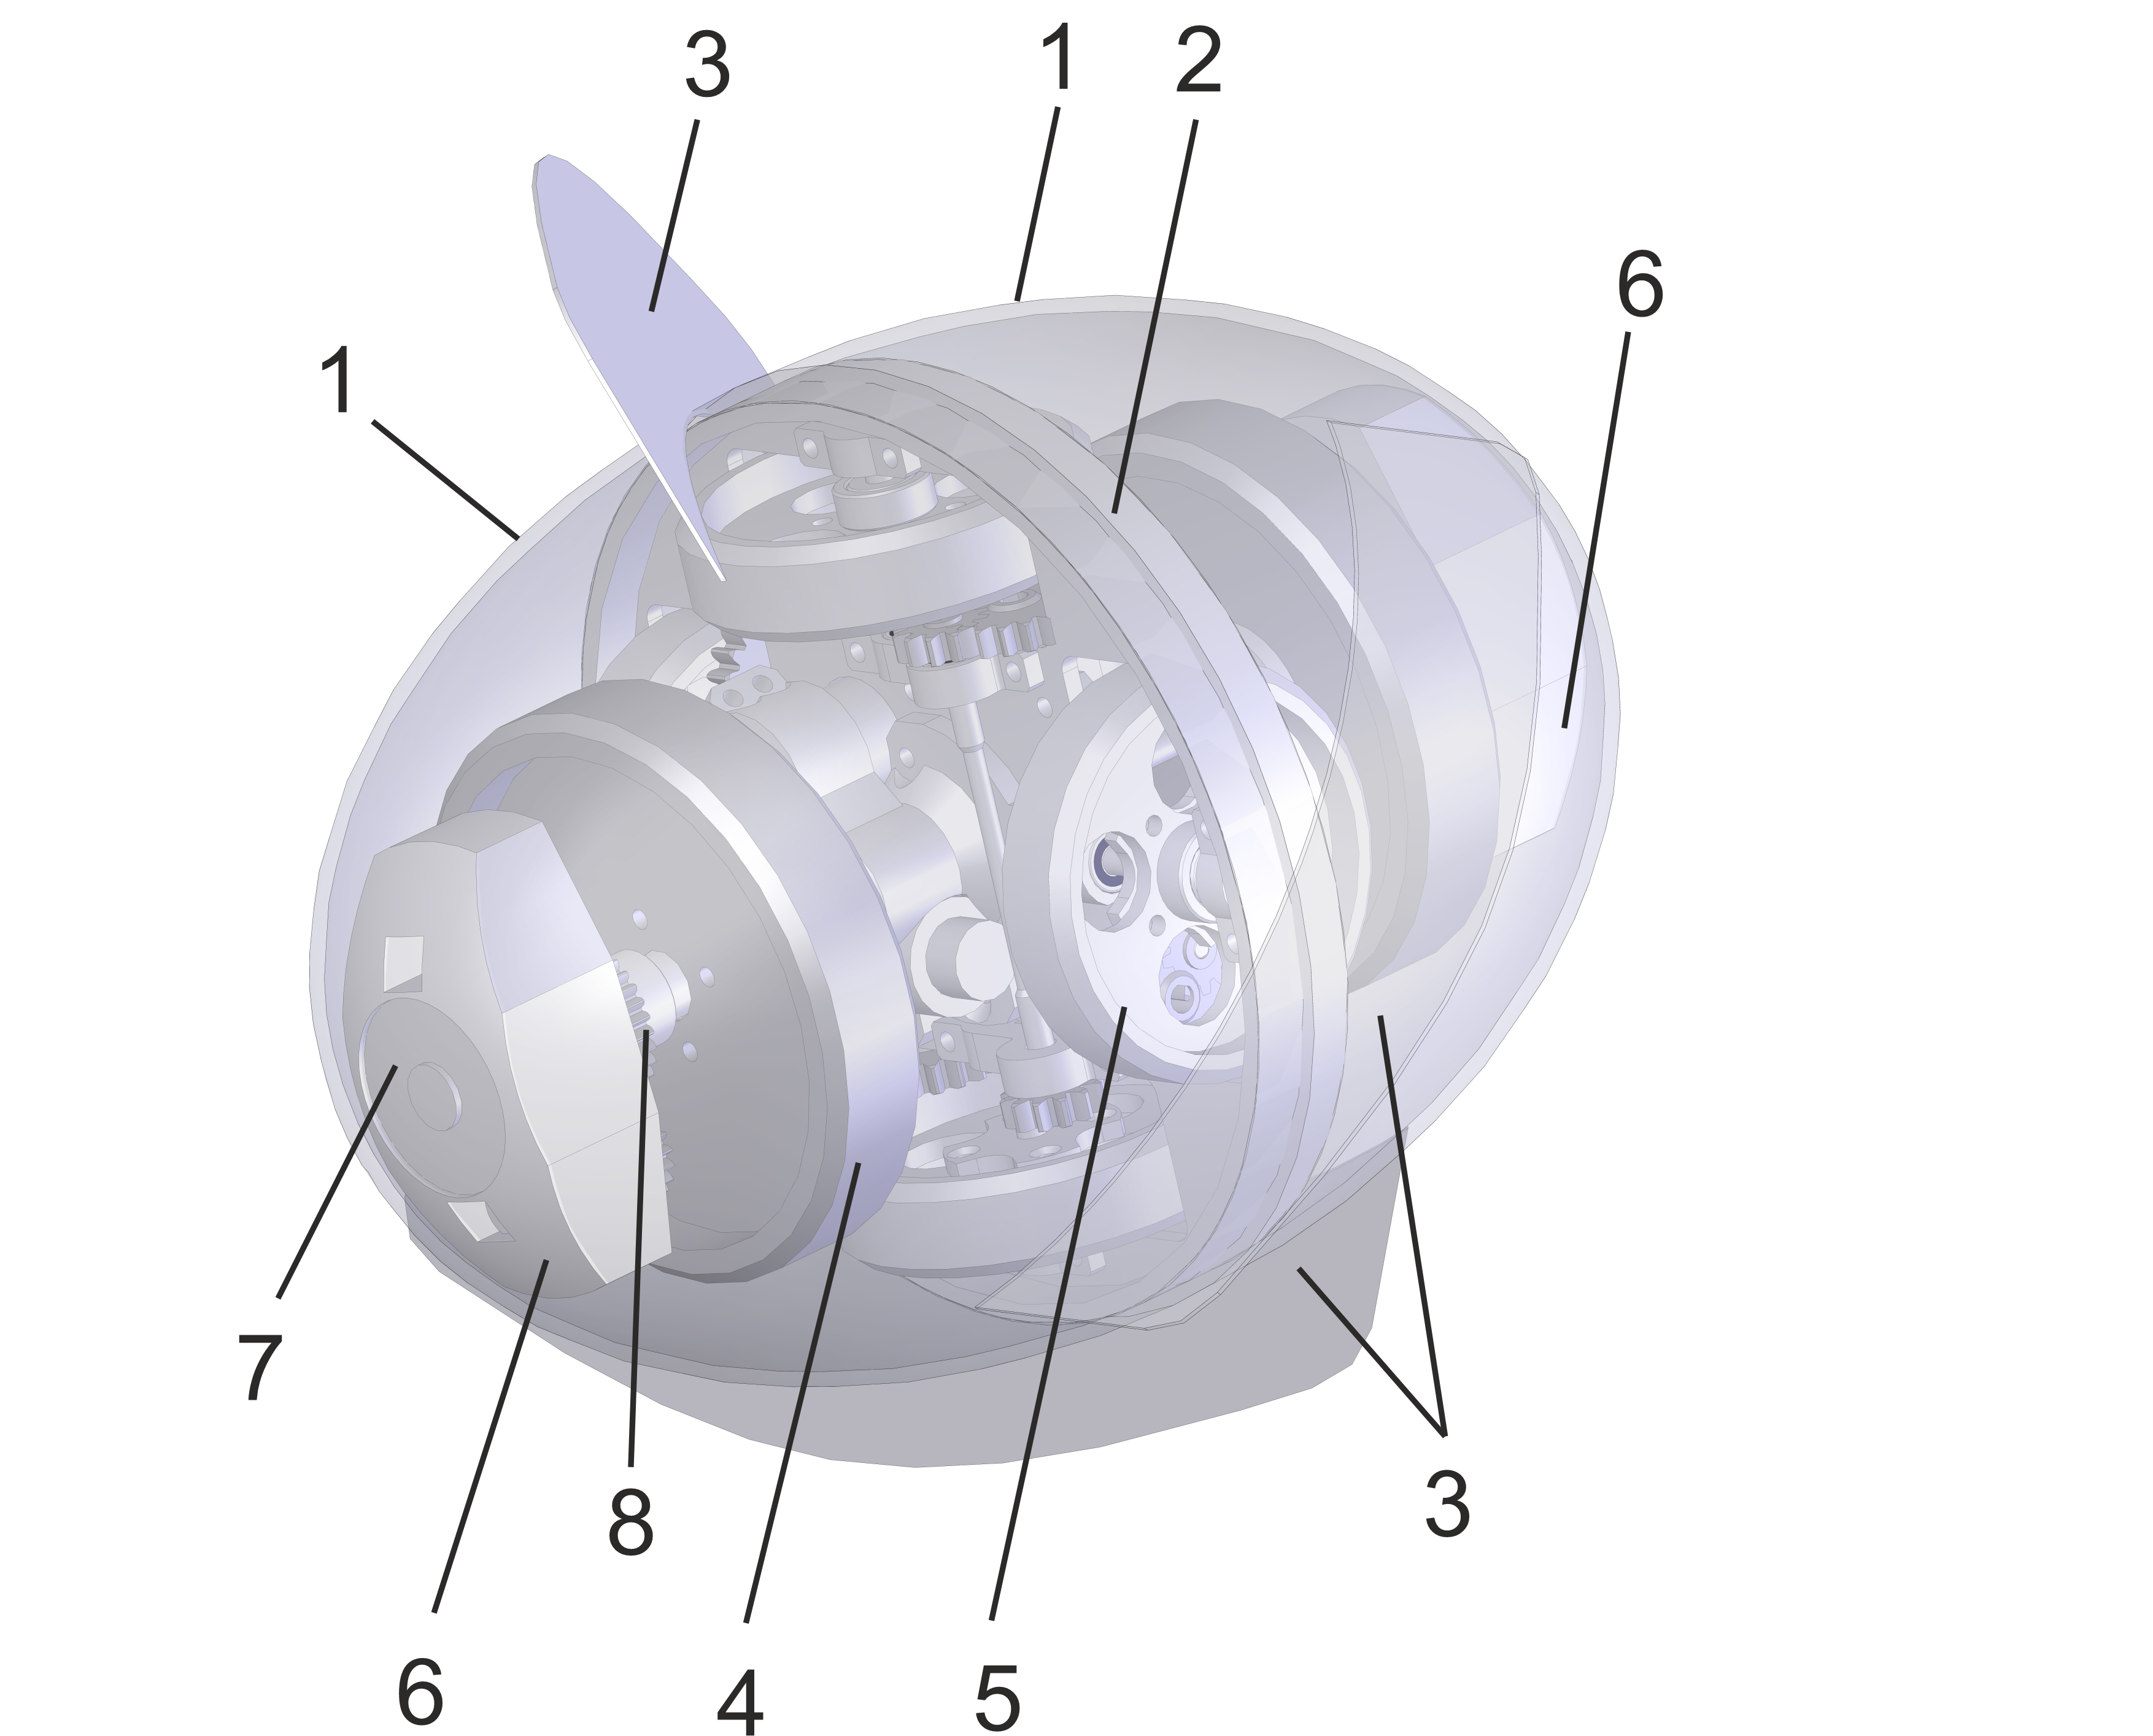
\includegraphics[width=0.7\linewidth]{BPR_ScrewModel.png}%
	\caption{Конструкция и корпусные элементы экспериментальной модели безвинтового подводного робота}
	\label{constr_BPR}
\end{figure}

Размещение узлов на платформе выполнено таким образом, чтобы в максимальной степени обеспечить симметричное расположение масс относительно геометрического центра тела, а также по возможности обеспечить минимальное отклонение центра масс от геометрического.

Внутри корпуса робота установлены три пары роторов (далее система роторов) таким образом, что оси роторов расположены под углом $90^\circ$ по отношению друг к другу. Ось одной из пар роторов направлена вдоль оси вращения эллипсоида, а две другие пары расположены в экваториальной плоскости. Обеспечение точного управляющего воздействия $\omega_k (t)$ осуществляется с помощью встроенных в приводы датчиков обратной связи (энкодеров). Система роторов подводного робота включает пару роторов большего размера 4, и двух пар роторов меньшего размера 5. Большие роторы 4 установлены симметрично относительно платформы 2 на одной общей оси. Две пары роторов меньшего размера 5, расположенны в экваториальной плоскости (по направлениям осей) и перпендикулярны друг другу. Оси малых роторов выполнены отдельно для каждого маховика и установлены соосно на некотором расстоянии друг от друга. Малые роторы соединены кинематически попарно с помощью промежуточных (дополнительных) осей и зубчатых пар таким образом, что их вращение происходит также, как если бы они были на одной общей оси.

Для погружения робот оснащен механизмом регулировки плавучести. Он состоит из двух одинаковых модулей плавучести 6, размещенных и закрепленных внутри полуоболочек в наиболее удаленных частях относительно платформы. Модули плавучести имеют в своем составе поворотный пневмоцилиндр 7 с приводом 8 на основе микроэлектродвигателя с редуктором. Полости пневмоцилиндра --- воздушная и жидкостная имеют каналы, соединяющие их соответственно с внутренней полостью и внешней средой. К выходному валу электродвигателя подсоединен редуктор с передаточным отношением 75:1, далее передача вращения от редуктора к пневмоцилиндру осуществляется с помощью пары шестерен с передаточным отношением 5.75:1. Характеристики двигателя представлены в таблице~\ref{tabMicroMotor}. 

\begin{table}[h]
	\centering
	\caption{Характеристики двигателя модуля плавучести}\label{tabMicroMotor}
	\begin{tabular}{|l|c|}
		\hline
		Номинальное напряжение питания & 6 В \\ \hline
		Передаточное отношение редуктора & 75:1 \\ \hline
		Момент на валу & 0.06 Нм\\ \hline
		Максимальная скорость вращения & 180 об/мин \\ \hline
		Ток холостого хода & 20 мА\\ \hline
		Пусковой ток & 360 мА \\ \hline
	\end{tabular}
\end{table}

Пневмоцилиндр используется фирмы EasyElec, модель CRB2BS20-270SEZ. Характеристики поворотного пневмоцилиндра приведены в таблице~\ref{tabPnevmo}. Фото пневмоцилиндра представлено на рисунке~\ref{Pnevmo}.

\begin{table}[h]
	\centering
	\caption{Характеристики пневмоцилиндра EasyElec CRB2BS20-270SEZ}\label{tabPnevmo}
	\begin{tabular}{|l|c|}
		\hline
		Производитель &	EasyElec \\ \hline
		Угол поворота & 270$^{\circ}$ \\ \hline
		Объем полости & 0.000041 м$ ^3 $ \\ \hline
		Минимальное давление & 0.15 МПа \\ \hline
		Максимальное давление & 0.7 МПа \\ \hline
		Размер резьбы на входных каналах & М5х0.8 \\ \hline
		Внешний диаметр & 40 мм\\ \hline
		Диаметр вала & 5 мм \\ \hline
	\end{tabular}
\end{table}

\begin{figure}[h]
	\centering
	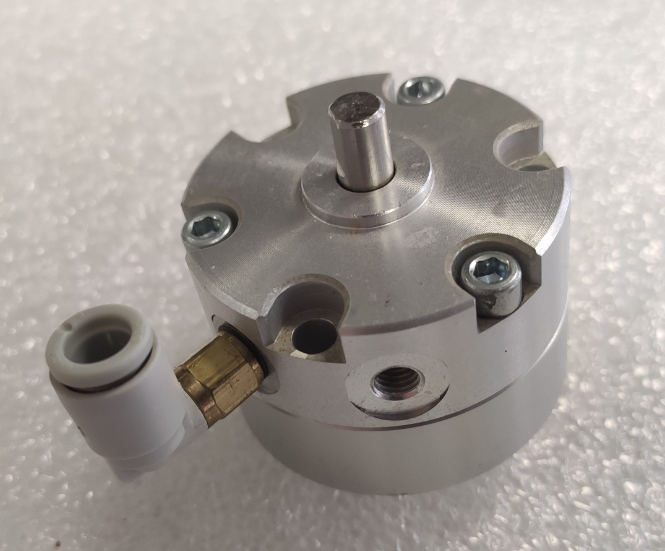
\includegraphics[width=0.4\linewidth]{Pnevmo.png}%
	\caption{Фото пневмоцилиндра EasyElec CRB2BS20-270SEZ}
	\label{Pnevmo}
\end{figure}

Конструкция модуля плавучести представлена на рисунке~\ref{FloatModule}.

\begin{figure}[!ht]
	\begin{minipage}[h]{0.5\linewidth}
		\center{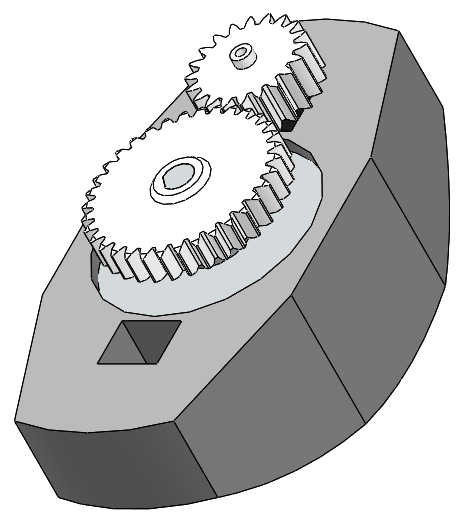
\includegraphics[width=0.8\linewidth]{FloatModule.png} \\ }
	\end{minipage}
	\hfill
	\begin{minipage}[h]{0.5\linewidth}
		\center{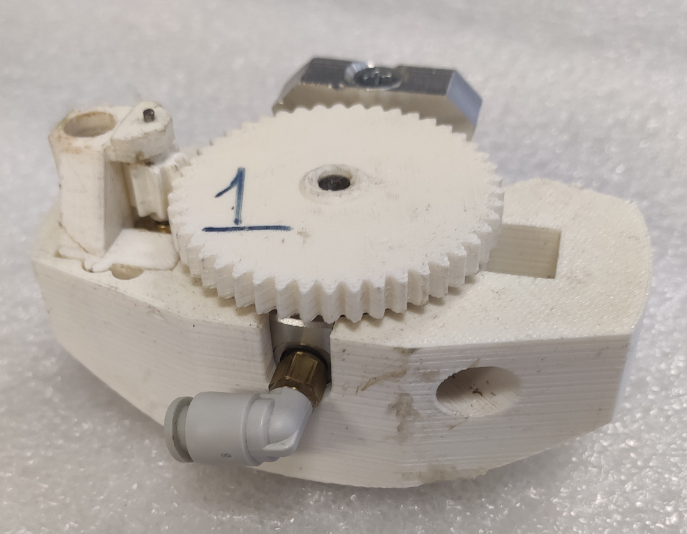
\includegraphics[width=0.9\linewidth]{FloatModuleReal.png} \\ }
	\end{minipage}
	\caption{Конструкция модуля плавучести}
	\label{FloatModule}
\end{figure}

Характеристики безвинтового подводного робота с внутренними роторами разработанной конструкции представлены в таблице~\ref{tabCharBPR}.
% : масса оболочки: $2.923$ кг; момент инерции маховиков большего размера: $7.491\cdot10^{-4}$ кг$\cdot$м; масса маховиков большего размера: $0.903$ кг;	момент инерции маховиков меньшего размера: $0.491\cdot10-4$ кг$\cdot$м;	масса маховиков меньшего размера: $0.337$ кг.

\begin{table}[h]
	\centering
	\caption{Характеристики безвинтового подводного робота с внутренними роторами}\label{tabCharBPR}
	\begin{tabular}{|l|c|}
		\hline
		Масса оболочки	&	$2.923$ кг 	\\ \hline
		Масса большого ротора &	$0.903$ кг	\\ \hline
		Масса малого ротора &	$0.337$ кг \\ \hline
		Момент инерции большого ротора 	& $7.491\cdot10^{-4}$ кг$\cdot$м \\ \hline
		Момент инерции малого ротора &  $0.491\cdot10-4$ кг$\cdot$м\\ \hline
	\end{tabular}
\end{table}

Фотографии робота в сборе и без половины оболочки представлены на рисунке~\ref{Photo_BPR}. 

\begin{figure}[h]
	\centering
	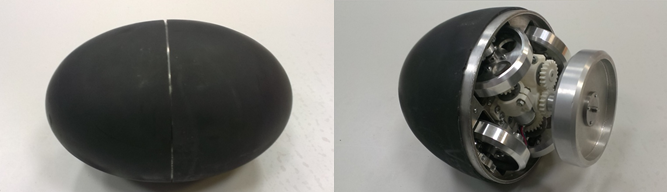
\includegraphics[width=0.9\linewidth]{Photo_BPR.png}%
	\caption{Фотографии безвинтового подводного робота}
	\label{Photo_BPR}
\end{figure}

Для придания роботу формы винтового тела к оболочке крепятся 3 лопасти. Полученное винтовое тело имеет диаметр винта 300 мм, угол наклона лопасти гребного винта к оси вращения эллипсоида --- 45$^{\circ}$.

\begin{figure}[h]
	\centering
	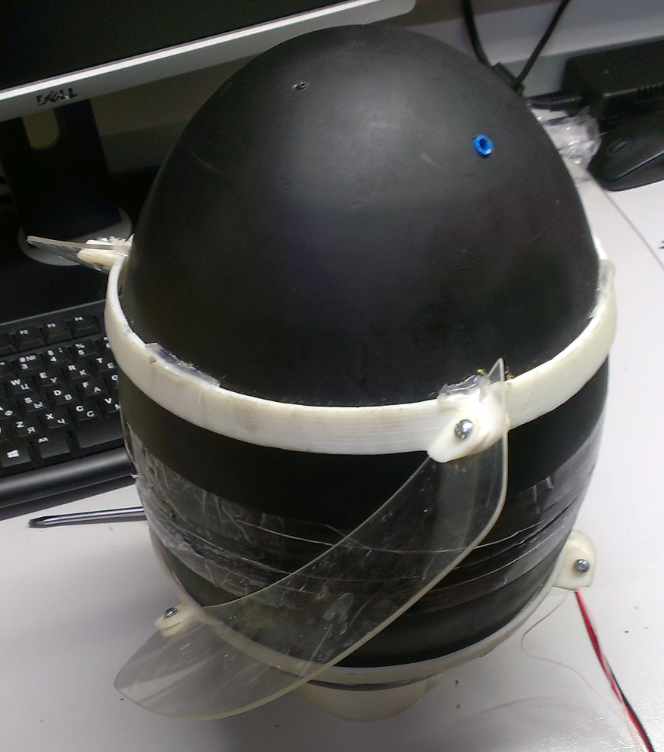
\includegraphics[width=0.4\linewidth]{BPR_Screw.png}%
	\caption{Фотографии безвинтового подводного робота с лопастями}
	\label{Photo_BPR_Screw}
\end{figure}


Для приведения в движение системы роторов каждая из пар роторов оснащена высокомоментными мотор-редукторами, которые установлены в соответствующих опорах на платформе. Кинематическая схема передачи вращения от двигателей к роторам представлена на рисунке~\ref{KinemBPR}.

\begin{figure}[h]
	\centering
	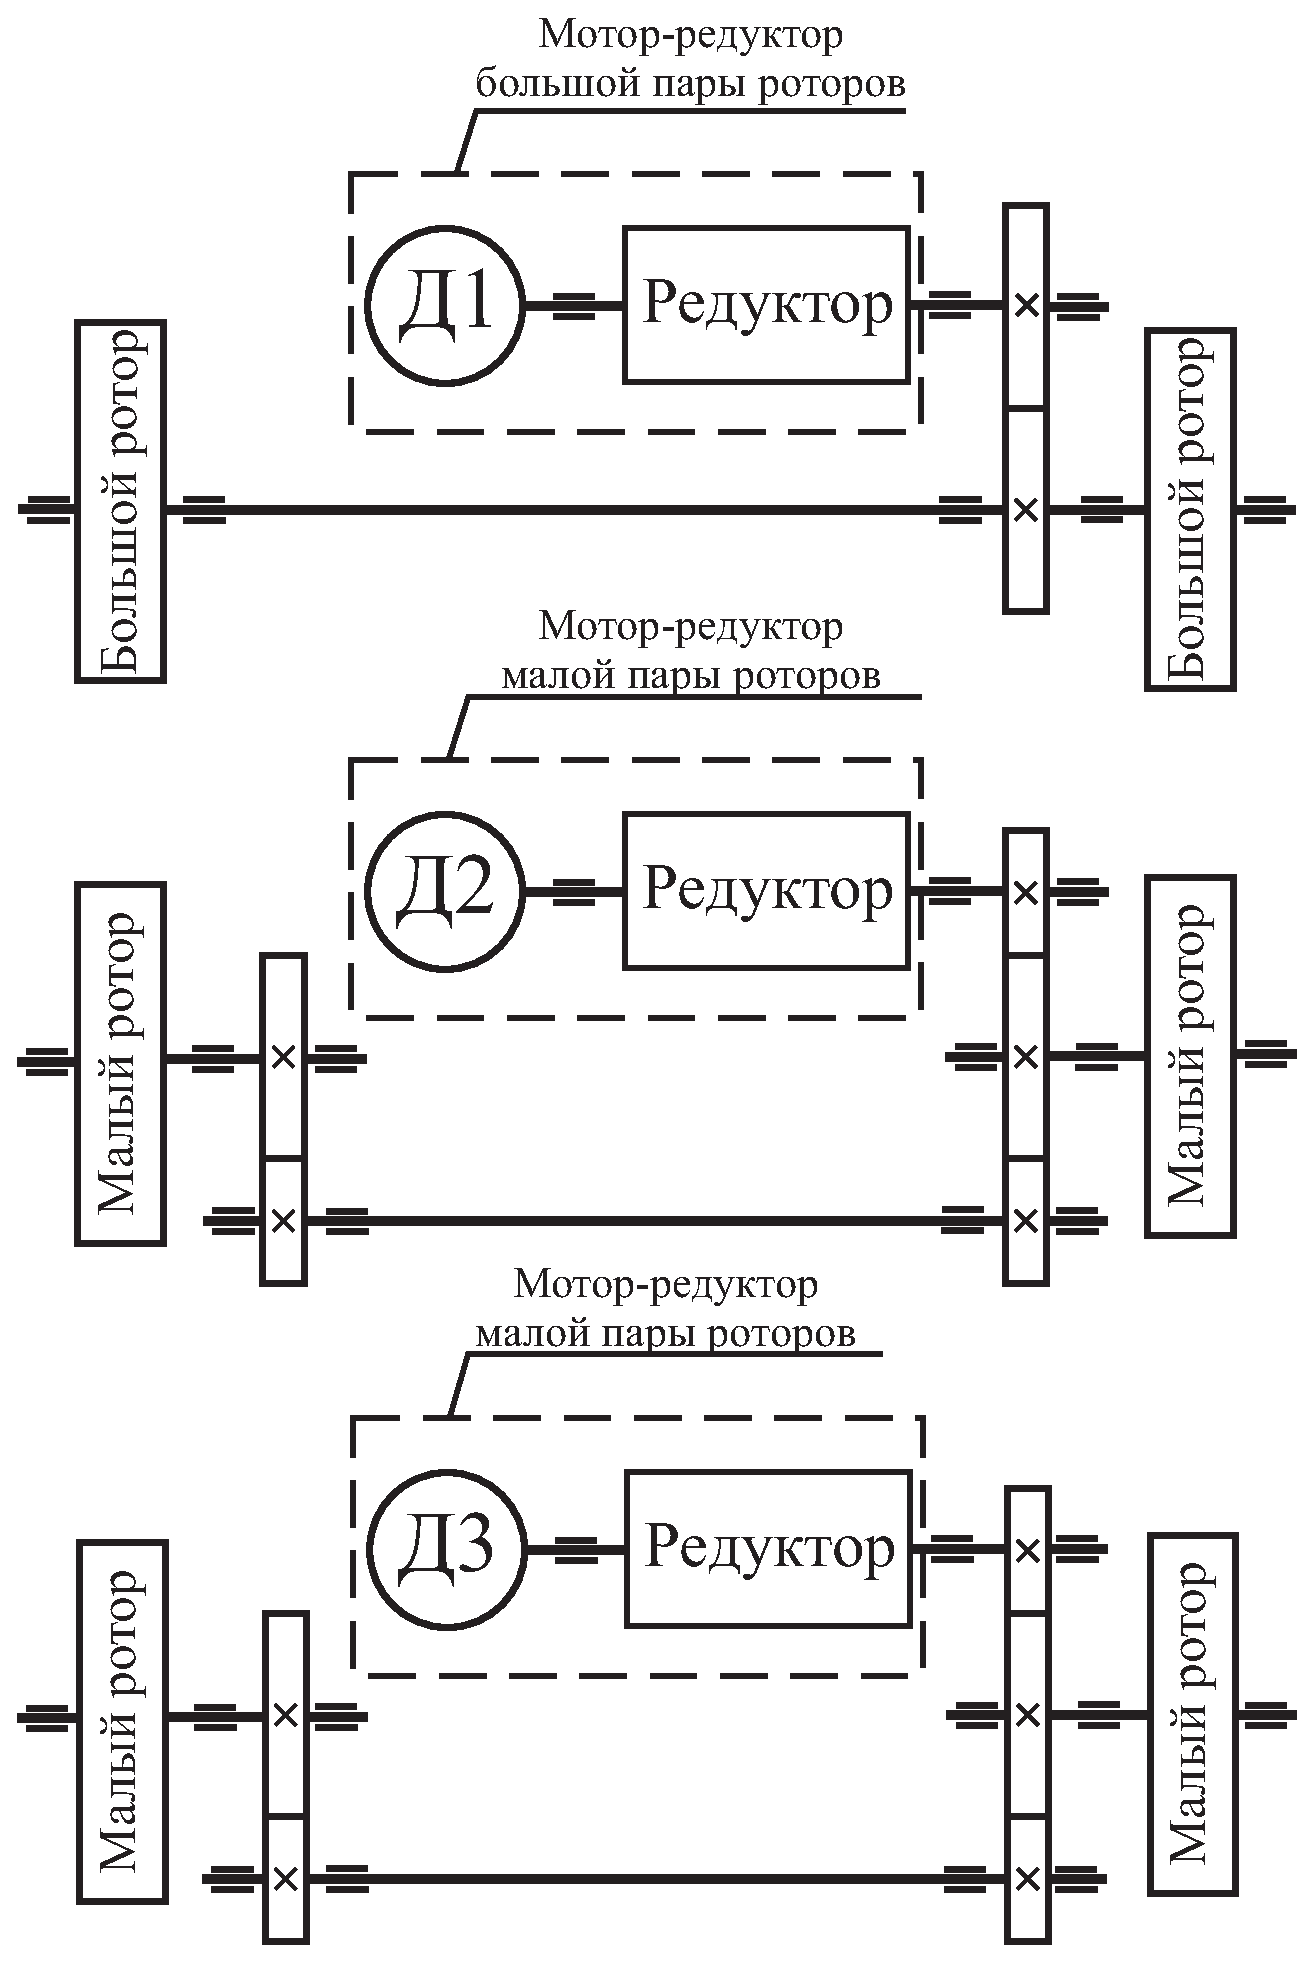
\includegraphics[width=0.6\linewidth]{KinemBPR.eps}%
	\caption{Кинематическая схема передачи вращения от двигателей к роторам}
	\label{KinemBPR}
\end{figure}

В качестве двигателя использовался мотор-редуктор с энкодером внешним диаметром 25 мм (см. рисунок~\ref{MotorBPR}). Характеристики двигателя представлены в таблице~\ref{tabMotor}. 

\begin{table}[h]
	\centering
	\caption{Характеристики двигателя}\label{tabMotor}
	\begin{tabular}{|l|c|}
		\hline
		Номинальное напряжение питания & 12 В \\ \hline
		Передаточное отношение редуктора & 47:1 \\ \hline
		Момент на валу & 0.6 Нм\\ \hline
		Максимальная скорость вращения & 160 об/мин \\ \hline
		Ток холостого хода & 200 мА\\ \hline
		Пусковой ток & 2.1 А \\ \hline
	\end{tabular}
\end{table}

\begin{figure}[h]
	\centering
	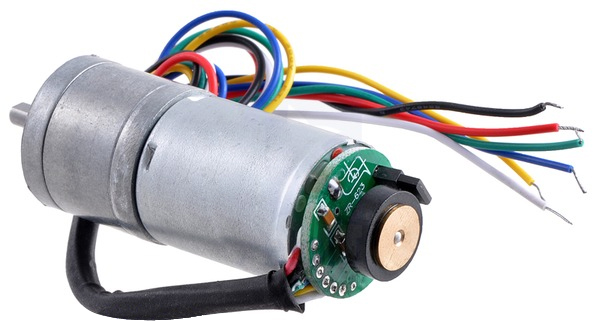
\includegraphics[width=0.5\linewidth]{Motor.jpg}%
	\caption{Мотор-редуктор фирмы Pololu с энкодером}
	\label{MotorBPR}
\end{figure}


Пара больших роторов расположена на оси, совпадающей с большей осью эллипсоида. Двигатель расположен параллельно этой оси и передача вращения от двигателя к роторам происходит через пару шестерен с 20 зубьями и передаточным отношением 1:1. 3Д-модель данной конструкции представлена на рисунке~\ref{BigRotorsBPR}.

\begin{figure}[h]
	\centering
	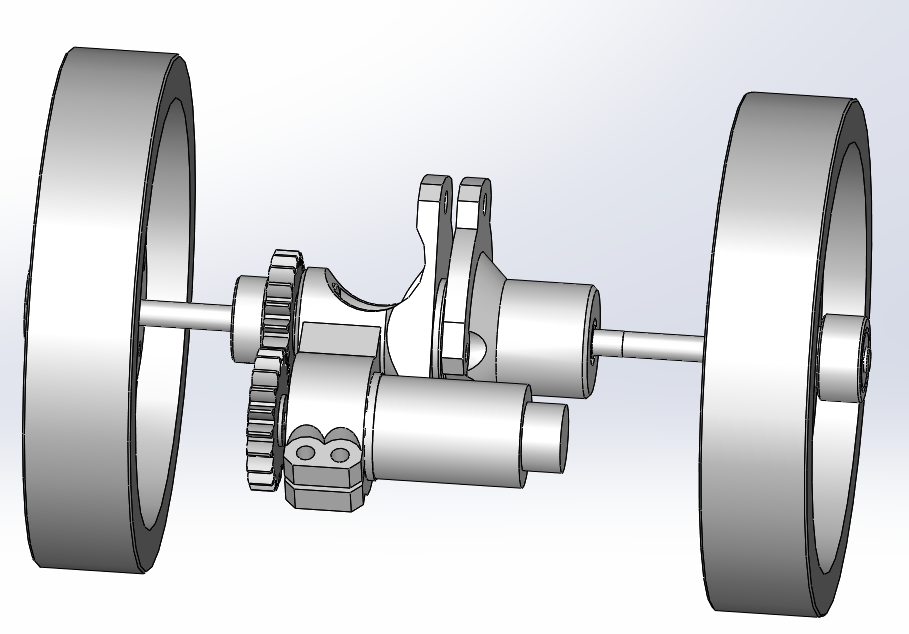
\includegraphics[width=0.5\linewidth]{BigRotorsBPR.png}%
	\caption{3Д-модель конструкции для передачи вращения от двигателя к паре больших роторов}
	\label{BigRotorsBPR}
\end{figure}

Для передачи вращения от двигателей к малым роторам используются промежуточные оси и шестерни на 12 и 20 зубьев (см. рисунок~\ref{KinemBPR}). Передаточное отношение между двигателем и каждым малым ротором составляет 1.6:1. 3Д-модель конструкции для передачи вращения от двигателя к одной паре малых роторов представлена на рисунке~\ref{SmallRotorsBPR}. Для второй пары малых роторов конструкция передачи вращения аналогичная.

\begin{figure}[!ht]
	\begin{minipage}[h]{0.5\linewidth}
		\center{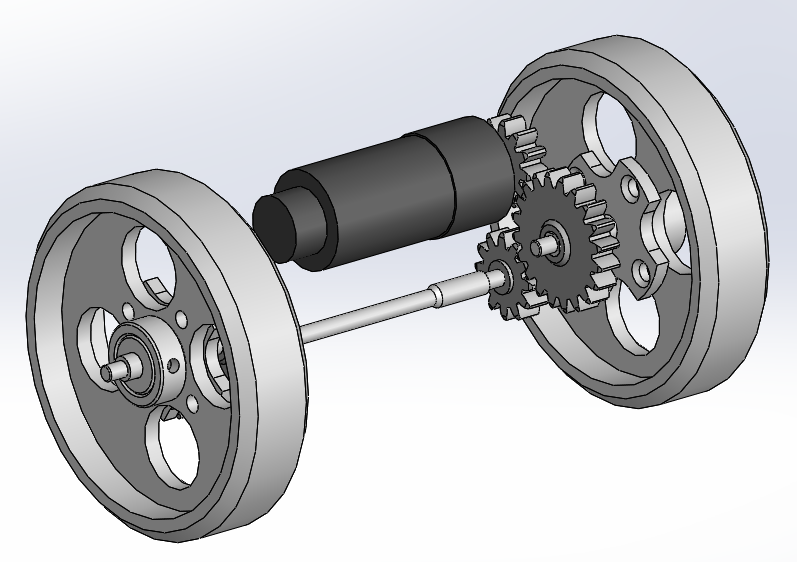
\includegraphics[width=0.8\linewidth]{SmallRotorsBPR1.png} \\ }
	\end{minipage}
	\hfill
	\begin{minipage}[h]{0.5\linewidth}
		\center{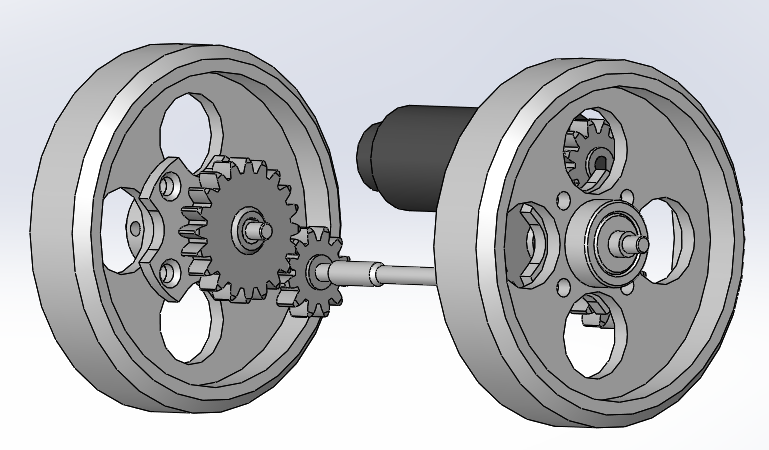
\includegraphics[width=0.9\linewidth]{SmallRotorsBPR2.png} \\ }
	\end{minipage}
	\caption{3Д-модель конструкции для передачи вращения от двигателя к паре малых роторов}
	\label{SmallRotorsBPR}
\end{figure}

На рисунке~\ref{SmallRotorsBPR3} представлено расположение двух пар малых роторов с их двигателями и элементами для передачи вращения. На рисунке~\ref{AllRotorsBPR} представлено взаимное расположение всех роторов робота.

\begin{figure}[h]
	\centering
	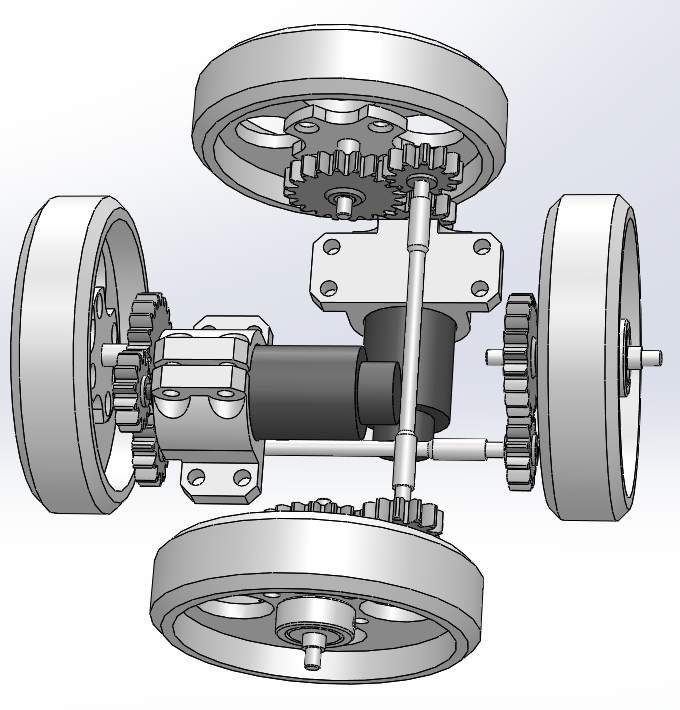
\includegraphics[width=0.5\linewidth]{SmallRotorsBPR3.png}%
	\caption{3Д-модель конструкции двух пар малых роторов с их двигателями и элементами для передачи вращения}
	\label{SmallRotorsBPR3}
\end{figure}

\begin{figure}[h]
	\centering
	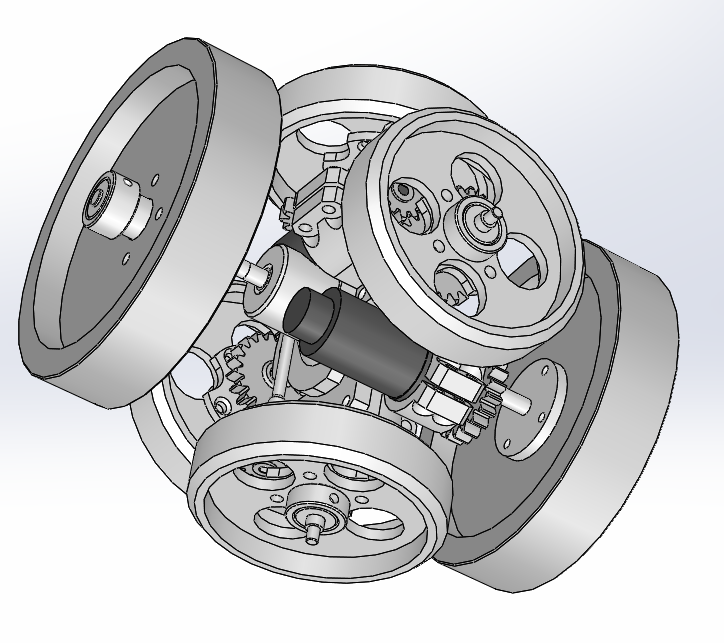
\includegraphics[width=0.5\linewidth]{AllRotorsBPR.png}%
	\caption{3Д-модель конструкции внутренних роторов безвинтового подводного робота}
	\label{AllRotorsBPR}
\end{figure}



В пространствах между большими и малыми роторами симметрично с двух сторон относительно платформы на панелях смонтированы модули питания 6, управления и связи.

В качестве модуля питания используется пара литий-полимерных (Li-Po) аккумуляторных батарей фирмы nVision %(см. рисунок~\ref{Accum}) 
с номинальным напряжением 7.4 Вольта, емкостью 450 мАЧ и максимальным выходным током до 13.5 Ампер. Аккумуляторные батареи соединены друг с другом параллельно.

%\begin{figure}[h]
%	\centering
%	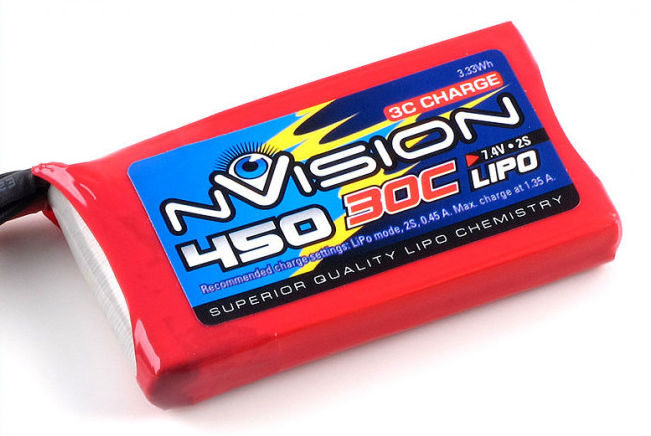
\includegraphics[width=0.5\linewidth]{Accum.png}%
%	\caption{Аккумуляторная батарея фирмы nVision}
%	\label{Accum}
%\end{figure}




\section{Описание системы управления безвинтового подводного робота с внутренними роторами}

Структурная схема системы управления безвинтового подводного робота с внутренними роторами, представлена на рисунке \ref{str_scheme}.

\begin{figure}[h!]
	\begin{center}
		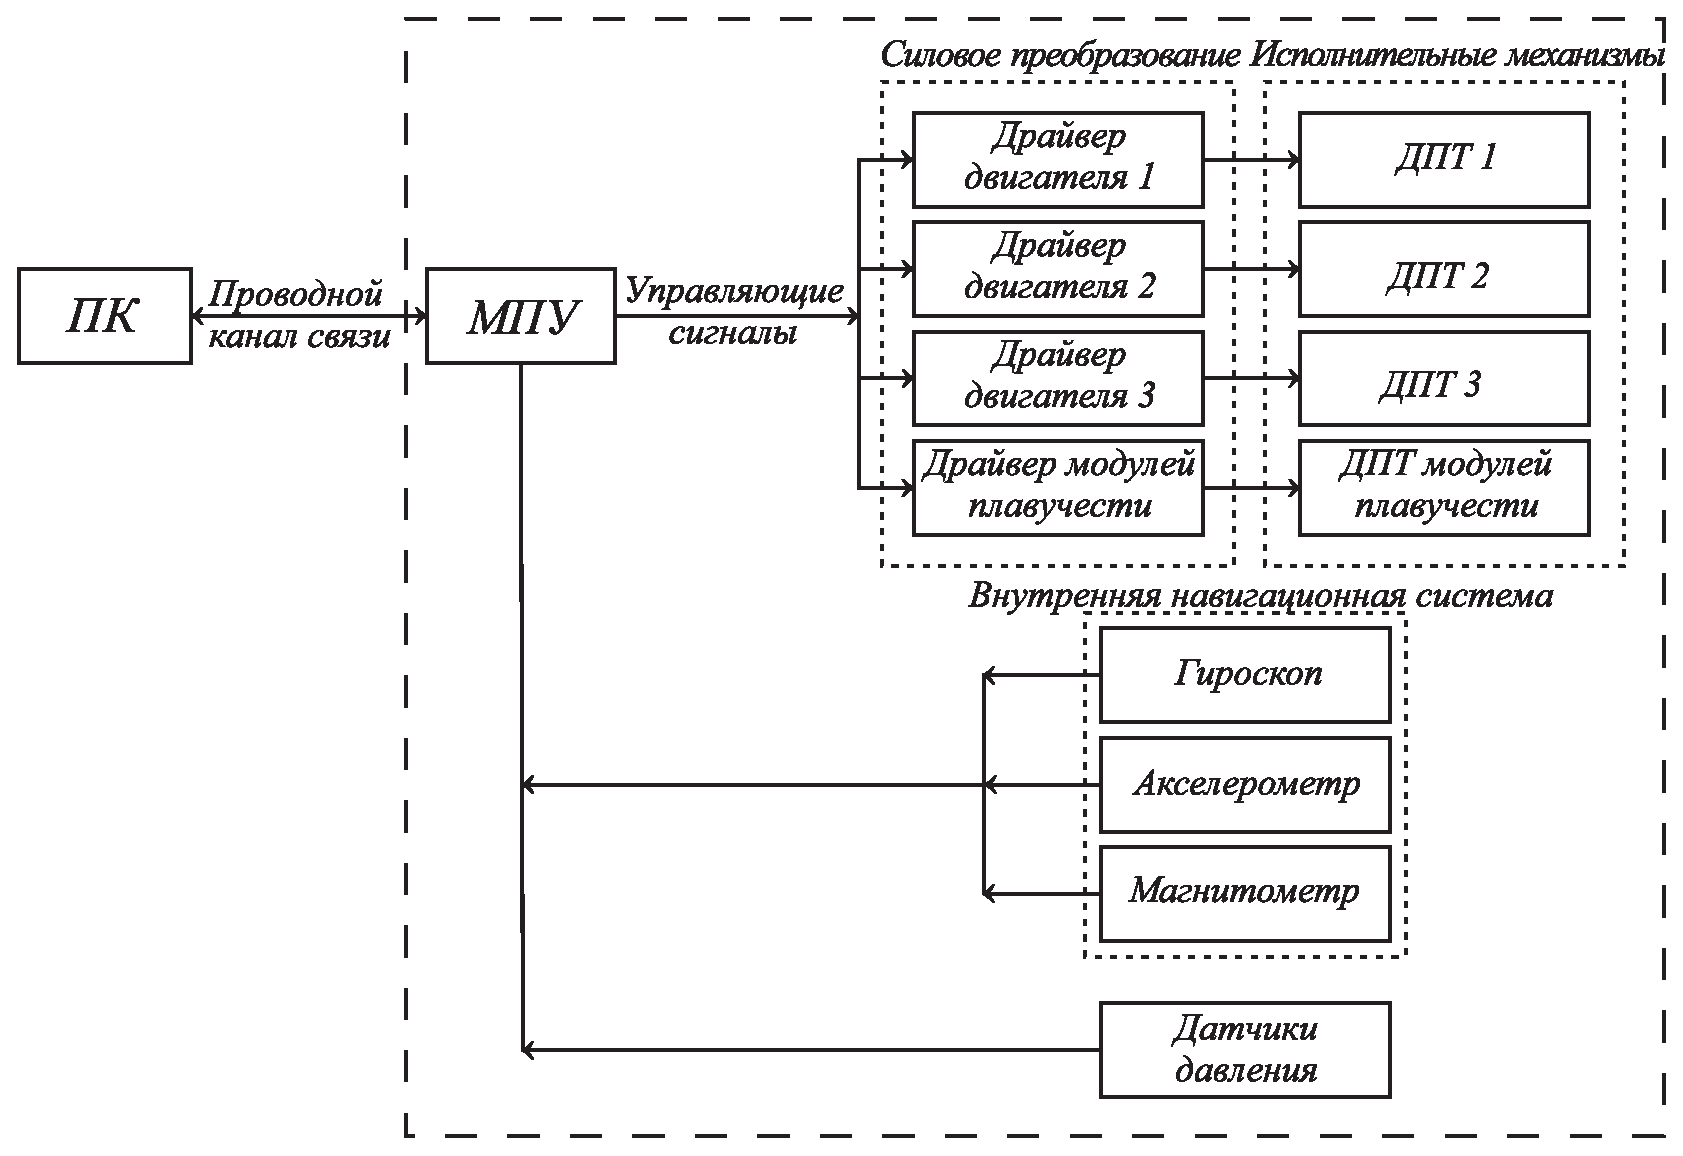
\includegraphics[width=0.8\linewidth]{StrSchemeBPR.eps}
		\caption{Структурная схема системы управления подводным роботом} \label{str_scheme}
	\end{center}
\end{figure}


\textbf{Описание микропроцессорного устройства (МПУ).} Центральным элементом системы управления является микроконтроллер LPC1768FBD100 фирмы NXP. Данный микроконтроллер имеет ядро ARM Cortex-M3, работает на частоте до 100 МГц и содержит большой набор различной периферии: 70 портов ввода-вывода; 4 таймера общего назначения с 6 выводами, имеющими возможность аппаратно формировать ШИМ-сигнал; контроллер прямого доступа в память, множество интерфейсов передачи данных. Характеристики микроконтроллера представлены в таблице~\ref{tabLpc}. В данной работе используется отладочная плата mbed NXP LPC1768 на основе вышеописанного микроконтроллера LPC1768FBD100 (см. рисунок~\ref{MbedLpc}).  Отладочная плата имеет 40-контактный DIP-форм-фактор; имеет всю необходимую обвязку элементов, необходимых для стабильной работы микроконтроллера; имеет DC-DC преобразователь, что позволяет питать плату напряжением в диапазоне от 5 до 15 вольт; позволяет загружать прошивку в микроконтроллер через USB интерфейс.

\begin{figure}[h]
	\centering
	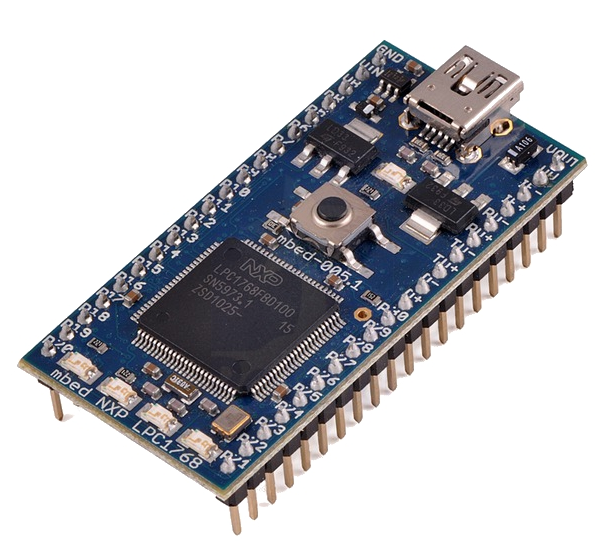
\includegraphics[width=0.4\linewidth]{MbedLpc.png}%
	\caption{Отладочная плата mbed NXP LPC1768}
	\label{MbedLpc}
\end{figure}

\begin{table}[h]
	\centering
	\caption{Характеристики микроконтроллера LPC1768FBD100}\label{tabLpc}
	\begin{tabular}{|l|c|}
		\hline
		Производитель &	NXP \\ \hline
		Корпус 	& LQFP100 \\ \hline
		Кол-во выводов 	& 100\\ \hline
		Архитектура ядра & Cortex-M3	\\ \hline
		Разрядность	& 32 бита\\ \hline
		Тактовая частота	& 100 МГц 	\\ \hline
		Оперативная память 	& 32 КБайт\\ \hline		
		Flash память & 512 КБайт\\ \hline		
		Количество входов / выходов & 70	\\ \hline
		Интерфейсы 	& Ethernet, USB, CAN, I2C, SPI, USART, I2S\\ \hline
		Разрешение АЦП & 12 бит\\ \hline
		Диапазон напряжений питания 	& 2.4...3.6 Вольт\\ \hline	
		Максимальная рабочая температура	&	$85^\circ$C 	\\ \hline
		Минимальная рабочая температура 	&	$-40^\circ$C \\ \hline	
	\end{tabular}
\end{table}

\textbf{Программа управления верхнего уровня.} Для управления безвинтовым подводным роботом с внутренними роторами на персональном компьютере разработано специальное программное обеспечение на языке C\#, окно которого представлено на рисунке~\ref{SoftHighLevel}. 

\begin{figure}[h]
	\centering
	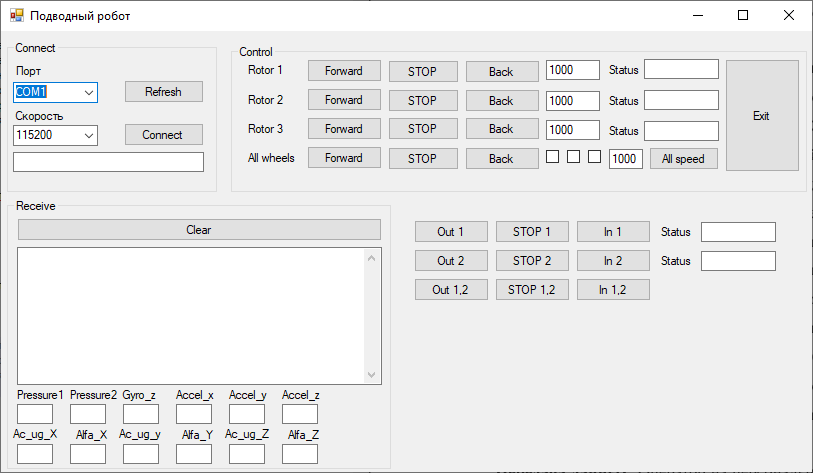
\includegraphics[width=1\linewidth]{SoftHighLevel.png}%
	\caption{Программа верхнего уровня для управления безвинтовым подводным роботом с внутренними роторами}
	\label{SoftHighLevel}
\end{figure}

В программе в группе элементов "Connect" реализованы функции выбора и подключения к необходимому СОМ-порту. В группе элементов "Control" реализованы функции управления двигателями роторов. Ниже расположены кнопки управления модулями плавучести. В группе элементов "Receive" расположено текстовое поле, в котором отображаются данные принимаемые с микроконтроллера робота, а так же маленькие текстовые поля для отображения отладочной информации: данные с датчиков давления, данные с гироскопа и акселерометра, углы ориентации робота.



\textbf{Передача данных.} Оператор на персональном компьютере (ПК, см. рисунок \ref{str_scheme}) задает команды управления подводным роботом. Команды передаются на микропроцессорное устройство (МПУ) по проводному или беспроводному (если робот находится на поверхности воды) каналу связи. Команды для двигателей представляют собой закодированные скорости вращения роторов или двигателей модулей плавучести. Протокол команд управления двигателями в общем виде представлен в таблице~\ref{tabProtokol}.

\begin{table}[h]
	\centering
	\caption{Протокол команд управления двигателями в общем виде для безвинтового подводного робота с внутренними роторами}\label{tabProtokol}
	\begin{tabular}{|c|c|c|c|}
		\hline 
		Длина пакета в байтах & Номер команды & Данные & Контрольная сумма \\ 
		\hline 
		1 байт & 1 байт & 4-6 байт & 2 байта \\ 
		\hline 
	\end{tabular} 
\end{table}

Для управления двигателями роторов используется команда 1, данными для этой команды выступают 6 байт: байт направления вращения (1 -- по часовой стрелке, 2 -- против часовой стрелки) и байт скорости вращения (об/мин) для каждого двигателя. После приема данной команды на микроконтроллере расчитывается текущий вектор гиростатического момента $\bK$, в виде которого задается управление в полученных математических моделях.

Для управления двигателями модулей плавучести используется команда 2, данными для которой выступают 4 байта: байт направления вращения и байт скорости вращения для каждого модуля плавучести.

Контрольная сумма рассчитывается по алгоритму CRC-16 CCITT.

%Передача данных для управления движением и получением дополнительной информации о состоянии системы может осуществляться по проводному и беспроводному вариантам связи. 

Проводной способ связи реализован с помощью переходника USB-USART на основе микросхемы CP2102, который подключается к USB-разъему персонального компьютера и позволяет создать виртуальный COM-порт. Для связи с микроконтроллером соответствующие выводы данного переходника подключены к выводам микроконтроллера, аппаратно поддерживающим интерфейс USART. Внешний вид переходника USB-USART представлен на рисунке~\ref{uartModules}а.

Беспроводной вариант связи реализован с помощью bluetooth-модуля HC-06, который работает аналогичным образом переходнику USB-USART: с микроконтроллером модуль НС-06 взаимодействует посредством интерфейса USART, а с компьютером bluetooth-модуль соединяется, используя профиль SPP (Serial Port Profile), что также позволяет создать виртуальный СОМ-порт и работать с ним. Внешний вид bluetooth-модуля HC-06 представлен на рисунке~\ref{uartModules}б.

\begin{figure}[!ht]
	\begin{minipage}[h]{0.5\linewidth}
		\center{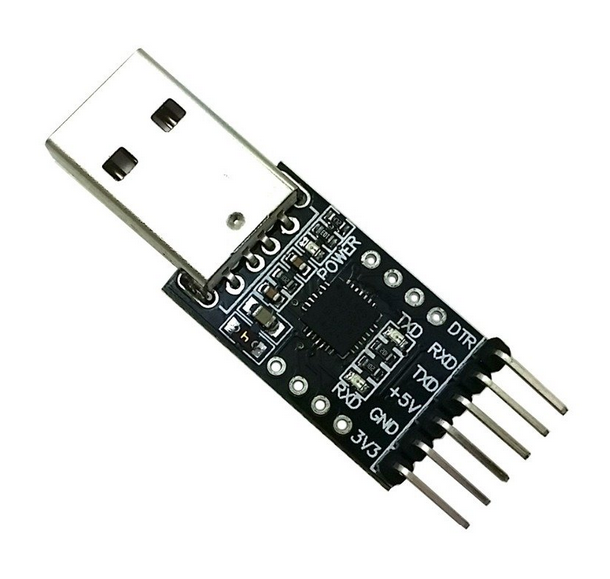
\includegraphics[height=0.7\linewidth]{Cp2102.png} }
	\end{minipage}
	\hfill
	\begin{minipage}[h]{0.5\linewidth}
		\center{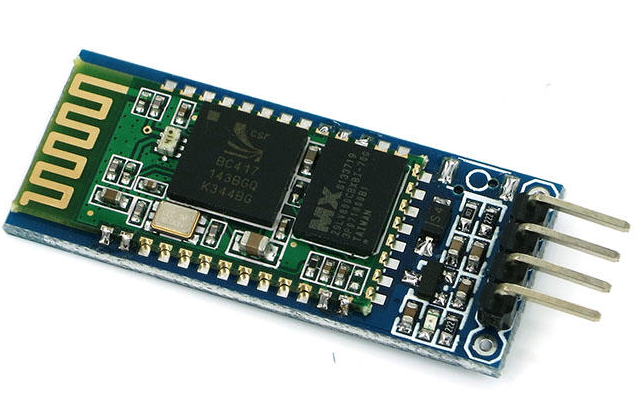
\includegraphics[height=0.6\linewidth]{HC-06.png} }
	\end{minipage}
	
	\begin{minipage}[h]{0.5\linewidth}
		\center{а}
	\end{minipage}
	\hfill
	\begin{minipage}[h]{0.5\linewidth}
		\center{б}
	\end{minipage}
	
	\caption{а) Модуль-переходник USB-USART. б) Bluetooth-модуль HC-06}
	\label{uartModules}
\end{figure}

\textbf{Управление двигателями.} Для управления отдельным двигателем роторов разработана схема, представленная на рисунке \ref{Control_system}.

\begin{figure}[h]
	\centering
	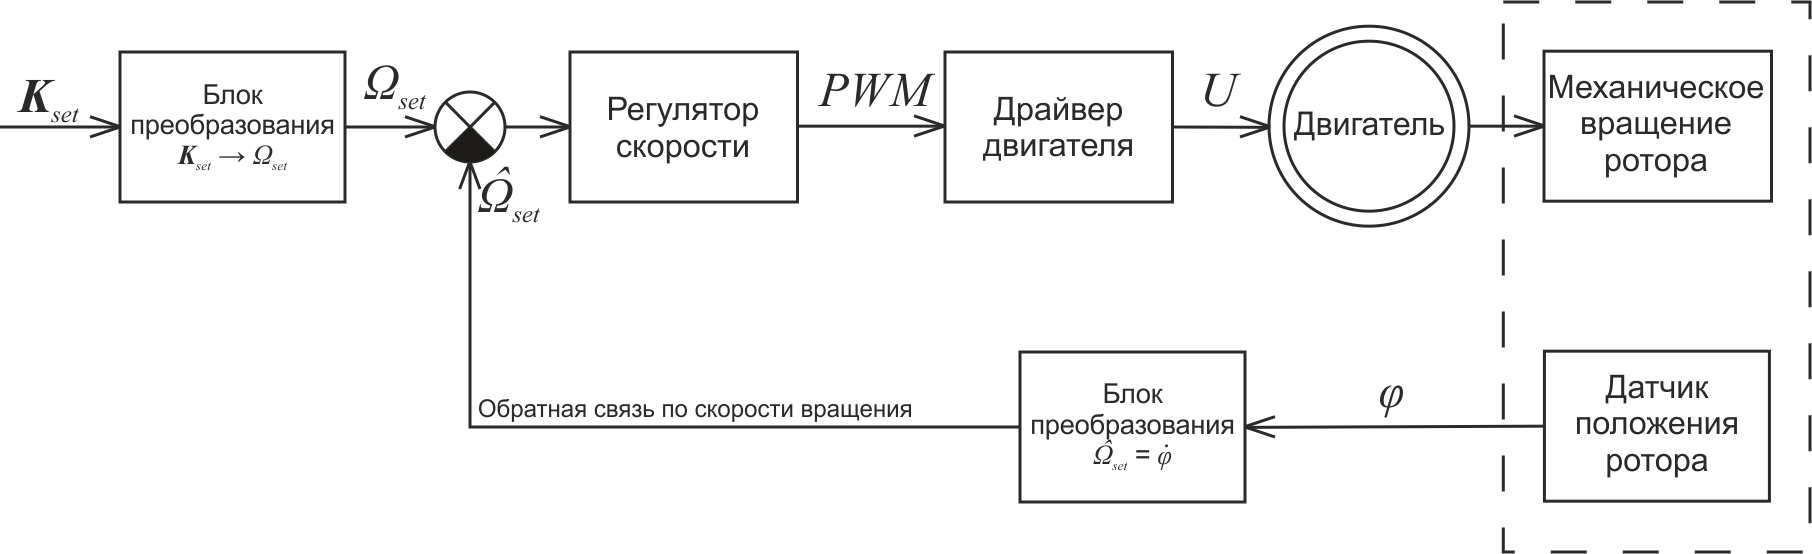
\includegraphics[width=0.9\linewidth]{Control_system.png}%
	\caption{Схема управления отдельным двигателем, где $\bK_{set}$ -- вектор внутреннего гиростатического момента; $\bOm_{set}$ -- угловая скорость вращения двигателя; $\hat{\bOm}_{set}$ -- фактическая скорость вращения двигателя; $PWM$ -- широтно-импульсная модуляция, рассчитанная для заданной скорости вращения; $U$ -- напряжение, подаваемое на двигатель; $\varphi$ -- фактическое положение ротора}
	\label{Control_system}
\end{figure}


Микропроцессор обрабатывает полученные данные и формирует управляющий сигнал, подаваемый на регулятор скорости, который представляет собой ПИ-регулятор. На выходе ПИ-регулятора получаем значение скважности ШИМ-сигнала, который формируется на выводе микроконтроллера и подается на драйвер двигателя. Драйвер двигателя усиливает сигнал с микроконтроллера, учитывая сигнал, определяющий направление вращения, и подает напряжение нужной формы непосредственно на двигатель постоянного тока.

Энкодер, расположенный на валу двигателя, фиксирует вращение вала двигателя и формирует сигнальные импульсы. Данный энкодер является инкрементальным, имеет два канала со смещением сигнала в четверть периода друг относительно друга, что позволяет определять направление вращения вала двигателя. Каждый канал формирует 12 импульсов на один оборот вала двигателя. Таким образом, используя два канала, считая переходы сигнала от низкого уровня к высокому и от высокого к низкому, можно получить 48 импульсов на один оборот вала двигателя и вычислить текущий угол поворота вала двигателя с точностью 7.5$ ^\circ$. Сигналы энкодера обрабатываются выводами микроконтроллера, настроенными на внешние прерывания.

Далее, получая изменение угла поворота вала двигателя во времени, можно рассчитать угловую скорость ротора, учитывая передаточные отношения передач между двигателем и ротором. Полученное значение является фактическим значением угловой скорости ротора и используется регулятором скорости в качестве обратной связи.

Для управления двигателями роторов используются драйверы двигателя постоянного тока VNH3SP30 фирмы STMicroelectronics. Данный драйвер обеспечивает выходной ток до 30 Ампер при напряжении от 5.5 до 36 Вольт. Драйвер содержит полномостовую схему силовых MOSFET-транзисторов, работающих в ключевом режиме, что позволяет управлять скоростью вращения и направлением вращения двигателя постоянного тока. Для данного драйвера была разработанна печатная плата, которая позволяет использовать микросхему драйвера и ее обвязку как отдельный модуль. Фото данного модуля представлено на рисунке~\ref{DriverPcb}. Характеристики данного драйвера представлены в таблице~\ref{tabVnh}

\begin{figure}[h]
	\begin{minipage}[h]{0.5\linewidth}
		\center{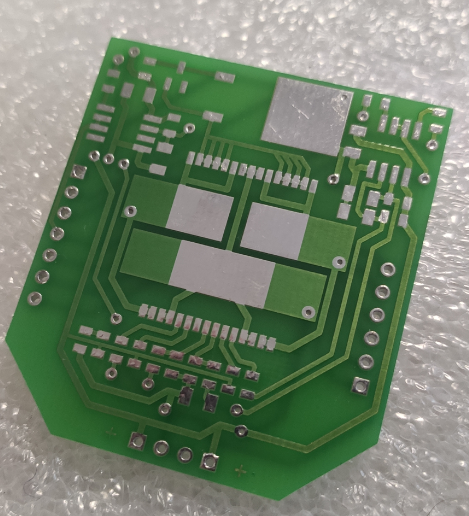
\includegraphics[height=0.8\linewidth]{DriverPcb2.png} }
	\end{minipage}
	\hfill
	\begin{minipage}[h]{0.5\linewidth}
		\center{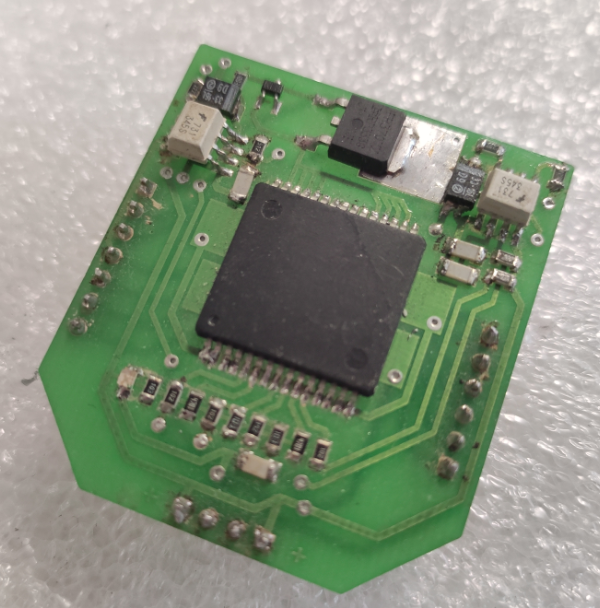
\includegraphics[height=0.8\linewidth]{DriverPcb.png} }
	\end{minipage}
	\vspace{2mm}
	\caption{Модуль управления двигателем постоянного тока на базе драйвера VNH3SP30}
	\label{DriverPcb}
\end{figure}

\begin{table}[h]
	\centering
	\caption{Характеристики драйвера двигателей постоянного тока VNH3SP30}\label{tabVnh}
	\begin{tabular}{|l|c|}
		\hline
		Количество каналов	&	1 	\\ \hline
		Максимальный пиковый ток нагрузки	&	45 А 	\\ \hline
		Максимальный непрерывный ток нагрузки  	&	30 А \\ \hline
		Максимальная частота ШИМ-сигнала 	& 10 кГц \\ \hline
		Напряжение низкого уровня управляющих сигналов &  0...1.5 В\\ \hline
		Напряжение высокого уровня управляющих сигналов &  3.25...36 В\\ \hline
		Напряжение нагрузки & 5.5...36 В \\ \hline
	\end{tabular}
\end{table}

Для управления двигателями модулей плавучести использовался драйвер двигателей постоянного тока на базе микросхемы TB6612FNG фирмы Toshiba (см. рисунок~\ref{DriverMini}), которая имеет внутри две полномостовые схемы MOSFET-транзисторов. С помощью одной микросхемы можно управлять двумя двигателями модулей плавучести. Характеристики данного драйвера представлены в таблице~\ref{tabDriverMini}.

\begin{figure}[h]
	\centering
	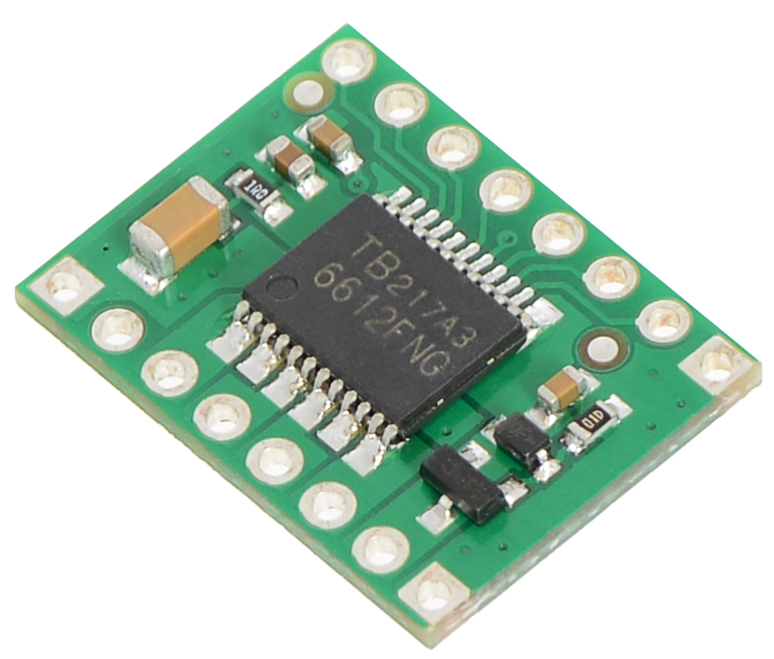
\includegraphics[width=0.4\linewidth]{DriverMini.png}%
	\caption{Драйвер двигателей постоянного тока на базе микросхемы TB6612FNG}
	\label{DriverMini}
\end{figure}

\begin{table}[h]
	\centering
	\caption{Характеристики драйвера двигателей постоянного тока TB6612FNG}\label{tabDriverMini}
	\begin{tabular}{|l|c|}
		\hline
		Количество каналов	&	2 	\\ \hline
		Максимальный пиковый ток нагрузки на канал	&	3 А 	\\ \hline
		Максимальный непрерывный ток нагрузки на канал 	&	1 А \\ \hline
		Максимальная частота ШИМ-сигнала 	& 100 кГц \\ \hline
		Напряжение управляющих сигналов &  2.7...5.5 В\\ \hline
		Напряжение нагрузки & 4.5...13.5 В \\ \hline
	\end{tabular}
\end{table}


\textbf{Описание датчиков.} Для определения ориентации робот имеет датчик на основе микросхемы MPU9250 (см. рисунок~\ref{Mpu9250}), который включает в себя трехосевой акселерометр, трехосевой гироскоп и трехосевой магнитометр. Данный датчик является цифровым, имеет на борту 16-битный аналого-цифровой преобразователь для оцифровки аналоговых данных с каждого сенсора. Датчик может быть подключен к микроконтроллеру по интерфейсам SPI или I2C. Характеристики датчика представлены в таблице~\ref{tabMpu}.

\begin{figure}[h]
	\centering
	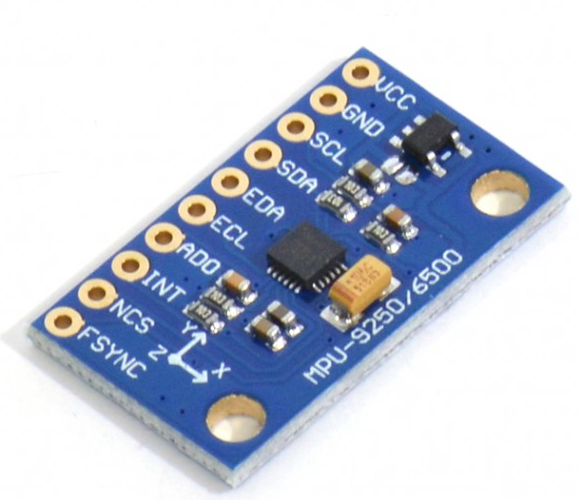
\includegraphics[width=0.3\linewidth]{Mpu9250.png}%
	\caption{Датчик MPU9250}
	\label{Mpu9250}
\end{figure}

\begin{table}[h]
	\centering
	\caption{Характеристики датчика MPU9250}\label{tabMpu}
	\begin{tabular}{|l|c|}
		\hline
		Рабочие диапазоны гироскопа & ±250, ±500, ±1000, ±2000 $^\circ$/с \\ \hline
		Чувствительность гироскопа & 131, 65.5, 32.8, 16.4 LSB/$^\circ$/c \\ \hline
		Рабочие диапазоны акселерометра & ±2, ±4, ±8, ±16 g\\ \hline
		Рабочий диапазон магнитометра & ±4800 мкТл\\ \hline
		Напряжение питания & 2.4...3.6 В\\ \hline
		Рабочий ток гироскопа & 3.2 мА\\ \hline
		Рабочий ток акселерометра & 450 мкА\\ \hline
		Рабочий ток магнитометра & 280 мкА\\ \hline
		Ток в режиме сна & 16 мкА \\ \hline
		Максимальная рабочая температура	&	$125^\circ$C 	\\ \hline
		Минимальная рабочая температура 	&	$-40^\circ$C \\ \hline
	\end{tabular}
\end{table}

Для расчёта ориентации объекта в пространстве по показаниям датчиков акселерометра, гироскопа и магнитометра использовался фильтр Маджвика (Madgwick filter)~\cite{Madgwick}. На выходе фильтра можно получить углы Эйлера, которые определяют углы крена, тангажа и рысканья. Точность определения углов ориентации объекта: 0.6$^\circ$ -- среднеквадратичное отклонение в неподвижном состоянии; 0.8$^\circ$ -- среднеквадратичное отклонение в подвижном состоянии. Данный фильтр может работать как с двумя (акселерометр и гироскоп) так и с тремя датчиками (акселерометр, гироскоп, магнитометр). При наличии магнитометра фильтр учитывает магнитные искажения и компенсирует смещения гироскопа. 
%На каждое обновление фильтра MARG необходимо выполнить 277 простых арифметических операций. 
Фильтр Маджвика можно использовать с частотой обновления от 10 Гц. Из-за невысокой вычислительной нагрузки и возможности работать на низких частотах дискретизации он подходит для вычисления углов ориентации на микроконтроллере. 

%\todo{привести мат аппарат, либо убрать про кватернионы и 277 арифметических оппераций}



Для контроля глубины робот оснащен двумя датчиками давления MPX5010GP фирмы NXP (см. рисунок~\ref{PressureSensor}), расположенными рядом с модулями плавучести. Датчик является аналоговым, максимальная величина измеряемого давления -- 10 кПа, что соотвествует 1019.78 мм глубины погружения в воде. Датчик подключается к входу 12-битного аналого-цифрового преобразователя (АЦП) микроконтроллера. Характеристики датчика представлены в таблице~\ref{tabPressure}.

\begin{figure}[h]
	\centering
	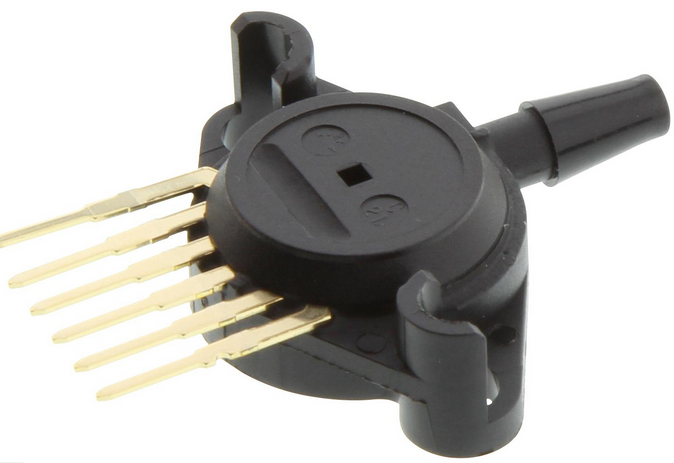
\includegraphics[width=0.5\linewidth]{PressureSensor.png}%
	\caption{Датчик давления MPX5010GP фирмы NXP}
	\label{PressureSensor}
\end{figure}

\begin{table}[h]
	\centering
	\caption{Характеристики датчика давления MPX5010GP фирмы NXP}\label{tabPressure}
	\begin{tabular}{|l|c|}
		\hline
		Максимальное рабочее давление	&	10 кПа 	\\ \hline
		Предельно допустимое давление & 40 кПа \\ \hline
		Чувствительность в жидкости	& 4.413 мВ/мм \\ \hline
		Время отклика 	& 1 мс \\ \hline
		Выходное напряжение при максимальном давлении	&  4.7 В\\ \hline
		Напряжение питания 	& 5 В\\ \hline	
		Потребляемый ток	& 5...10 мА\\ \hline	
		Точность	& 5\% \\ \hline
		Максимальная рабочая температура	&	$125^\circ$ C 	\\ \hline
		Минимальная рабочая температура 	&	$-40^\circ$ C \\ \hline
	\end{tabular}
\end{table}

%Рассчитаем минимальное изменение глубины, которое может воспринимать датчик давления. Так как опорное напряжение АЦП микроконтроллера -- 3.3 Вольта, для преобразования выходного сигнала датчика, имеющего максимальное значение в 4.7 вольта, использовался делитель напряжения на резисторах номиналами 10 кОм и 15 кОм. Коэффициент преобразования данного делителя напряжения -- 1.67, следовательно максимальное напряжение, поступающее на вход АЦП микроконтроллера, составит 2.81 В. АЦП, к которому подключены датчики давления является 12-ти разрядным с опорным напряжением 3.3 В. Поэтому разрешающая способность данного АЦП -- 3.2 мВ, а до делителя напряжения 5.12 мВ. Таким образом, можно определять изменение глубины на 1.16 мм.
Использование данного датчика давления в связке с микроконтроллером LPC1768 позволяет определять глубину до 1 метра с точностью 1.2 мм. 



\textbf{Плата управления.} Для размещения внутри оболочки безвинтового подводного робота была разработана плата управления с электронными компонентами специальной формы (см.рисунок~\ref{PCB_BPR}). Плата крепится к перегородке, расположенной в экваториальной плоскости эллипсоида. Через отверстие в центре платы проходит ось, на которой закреплены большие роторы. Вырезы по краям платы сделаны для четырех малых роторов.

\begin{figure}[h!]
	\begin{center}
		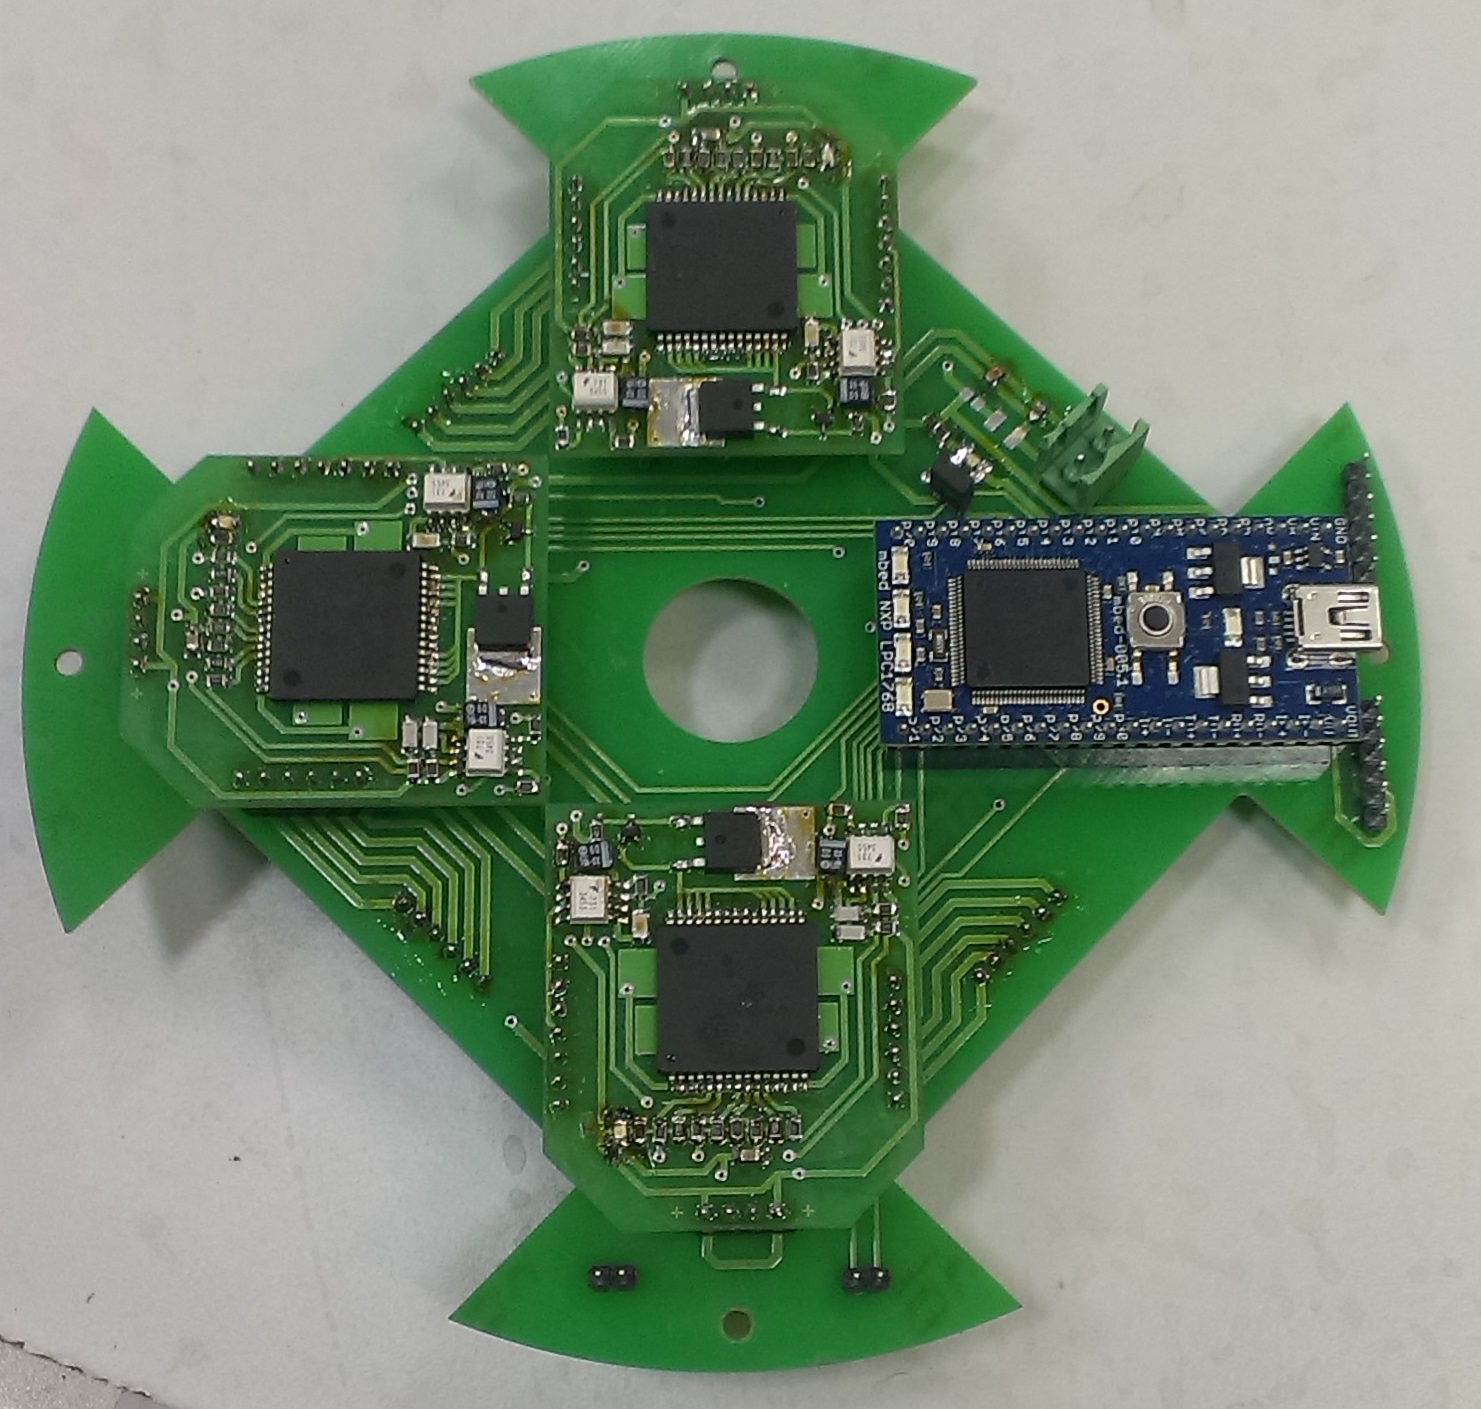
\includegraphics[width=0.8\linewidth]{PCB_BPR.png}
		\caption{Плата управления безвинтового подводного робота с внутренними роторами} \label{PCB_BPR}
	\end{center}
\end{figure}

%Управление осуществляется с персонального компьютера (ПК), для которого было разработано специальное программное обеспечение. Для управления роботом необходимо задать направления и скорости вращения каждого из роторов, а также время разгона до заданной скорости. Отдельно осуществляется управление модулями плавучести, которые отвечают за погружение робота.


\section{Выводы по главе}

В данной главе описана конструкция безвинтового подводного робота с внутренними роторами. Для симметричности конструкции вместо трех отдельных роторов робот имеет три пары роторов, в каждой паре роторы равноудалены от центра всей системы. Ввиду ограничений размеров оболочки разработаны специальные кинематические схемы приведения в движение пар роторов. Разработана система управления роботом, описаны ее основные компоненты.










\clearpage